\subsection{The Plane Before Coordinates}

\begin{corebox}[Starting point]
At first there is only a Euclidean plane. No line has been selected as an axis,
no point has been selected as an origin, no orientation has been declared
positive, and no numerical scale has been imposed.
\end{corebox}

\begin{center}
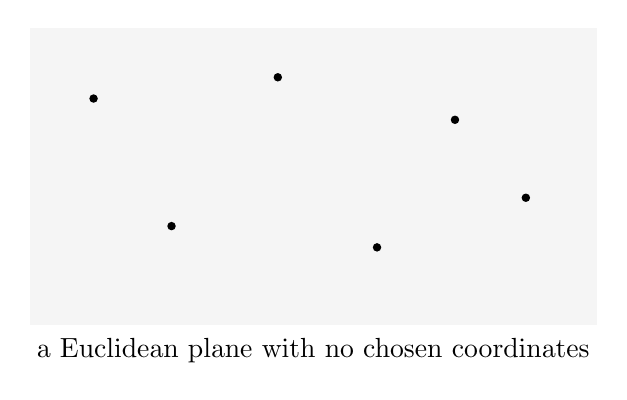
\begin{tikzpicture}[scale=0.9]
    \fill[gray!8] (-4,-2.1) rectangle (4,2.1);
    \foreach \x/\y in {-3.1/1.1,-2.0/-0.7,-0.5/1.4,0.9/-1.0,2.0/0.8,3.0/-0.3} {
        \fill (\x,\y) circle (1.7pt);
    }
    \node at (0,-2.45) {a Euclidean plane with no chosen coordinates};
\end{tikzpicture}
\end{center}

\begin{interpretationbox}[Coordinates are additional structure]
The Cartesian plane will be obtained by making a sequence of choices inside
this pre-existing geometry. Those choices do not change the points or lines;
they create a systematic numerical language for describing them.
\end{interpretationbox}
